\documentclass[sotsuron]{jcsie}
\usepackage[dvipdfmx]{graphicx}
\usepackage{float}

\title{ライブストリーミングに対応した分散ハッシュテーブルの検討}
\etitle{Title}
\author{沈 嘉秋}
\eauthor{Yoshiaki Shin}
\id{T18I917F}
\keywords{P2P, 分散ハッシュテーブル}
\ekeywords{hoge, hoge}

\begin{document}
\maketitle
\emaketitle
\pagenumbering{roman}
\begin{abstract}    
	分散ハッシュテーブルはファイル共有サービス等に応用され、
	すでに普及している一方で、
	近年はブロックチェーンの関連技術としても注目を集めている。
	分散ハッシュテーブルの中でもKademliaはその実装の容易さと
	ノードの出入りに対する耐性の強さから
	実用的なサービスへの応用が可能であり、
	多くのサービスで採用されている。
	近年、ライブストリーミングサービスの需要が高まっている
	一方で配信プラットフォームの事業者への依存が強く
	サービス利用者の立場は弱いものとなっている。
	そこで本論文では
	分散的なライブストリーミングサービスの基盤となる
	システムをKademliaを元に実装し、その評価を行った。
	Kademlia上で単純にライブストリーミングの実装を行う場合、
	非効率的な通信が発生するが、本論文の手法では、
	Kademliaネットワークを更に構造化することで
	非効率的な通信を削減することが可能となった。
	結果、分散的なライブストリーミングサービスの実装への
	足がかりを作ることが出来た。
\end{abstract}
\begin{eabstract}
	Here is abstract
	Here is abstract
	Here is abstract
	Here is abstract
	Here is abstract
	Here is abstract
	Here is abstract
	Here is abstract
	Here is abstract
	Here is abstract
	Here is abstract
	Here is abstract
	Here is abstract
	Here is abstract
\end{eabstract}
\tableofcontents
\pagenumbering{arabic}
\chapter{はじめに}
\section{背景}
近年、P2Pネットワーク技術がブロックチェーンなどによって再び注目を集めている。
最近ではブロックチェーン流行以前に流行していた
P2Pネットワーク技術を利用した分散型ファイル共有サービスと
組み合わせて開発されたサービスも見られる。\footnote{https://www.bittorrent.com/btt/}
分散型ファイル共有サービスは分散ハッシュテーブルという技術を用いて
実装されることがあり、分散型ファイル共有サービスの中でも
利用者の特に多いBitTorrentではKademliaという分散ハッシュテーブルを
用いて開発されている。
分散型ファイル共有サービスはこれまで、膨大なサーバリソースを持つ
大企業などでなければ実現できなかった、大規模かつ、高速な
ファイル共有を実現した。

近年Youtube Live や Twitch といった動画ライブストリーミングサービスが
家庭用ネットワークやモバイルネットワークの環境改善に伴い普及してきている。
しかし、これらのサービスは膨大なサーバリソースを持つ大企業などでなければ
実現できず、プラットフォーム事業者への依存が強く、
サービス利用者の立場は弱いものとなっており不健全な状態にある。

\section{目的}
分散ハッシュテーブルの中でもKademliaはその実装の容易さと
ノードの出入りに対する耐性の強さから実用的なサービスへの応用が可能
であるが、その一方でKademlia上で単純にライブストリーミングの実装を行う場合、
非効率的な通信が発生する。

そこで本論文では、分散型の動画ライブストリーミングサービスの基盤
となるシステムを、Kademliaをベースに改良し実装する。
成果物がWebブラウザとNode.jsで動作するライブラリとなるように開発を行う。

成果物ができるだけ多くのプラットフォームで動作するようにするために
P2P通信箇所にWebRTC \footnote{https://webrtc.org/}
を用いる。WebRTCはWebブラウザなどといったフロントエンド
環境とサーバーサイド環境の両方に対応した低遅延通信のための規格である。
またWebRTCは近年では、スマートフォンやパーソナルコンピュータに搭載されている
Webブラウザで動作する唯一のP2P通信規格でもある。

完成したライブラリを用いたベンチマークプログラムと
一般的なKademliaを用いたベンチマークプログラムをNode.js上で実行し
その性能や性質の比較を行い有用性などの検証を行う。
完成したライブラリを用いてWebブラウザ上で動作する
分散ライブ動画配信アプリのサンプルを開発し動作確認する。


\chapter{知識}
\section{分散ハッシュテーブル}
分散ハッシュテーブルとは、
あるデータとそのハッシュ値をペアとしたハッシュテーブルを
P2Pネットワーク上で複数のノードによって分散的に実装する技術である。
複数のノードにデータを分散配置を行うため適切な構造化を行う必要がある。
構造化には様々な手法が存在し、
ChordやKademliaといったさまざまな実装が存在する。
分散ハッシュテーブルの実装の優劣はデータの探索効率、
Churn耐性\footnote{ノードの出入りに対する耐性}、
実装の容易さなどによって付けられる。

\section{Kademlia}
Kademliaとは分散ハッシュテーブルの一種である。
高いChurn耐性を持つため、実用的なP2Pアプリケーションにて多く利用されている。
Kademliaはノード数Nのシステムにおいてデータを探索する際に
$O(\log(n))$ 回ノードへの通信を行う。

\subsection{採用例}
\begin{table}[H]
	\begin{tabular}{|l|l|}
		\hline
		サービス名 & 使用箇所 \\ 
		\hline
		Torrent         &              
		\begin{tabular}{l}
		magnetURLという機能を用いてファイルをダウンロードする際に\\
		目的のファイルを持っているノードを探索するのにKademliaを用いている。\\
		Torrentはアクティブユーザと転送量という点で見ると\\
		世界で最も成功したP2Pのシステムであり、\\
		そのシステムにKademliaはおおいに貢献していると言える。\\
	\end{tabular}\\ \hline
	Ethereum &
	\begin{tabular}{l}
		Node Discovery Protocol v4 というノードの探索プロトコルに用いられている. 
	\end{tabular}\\ \hline
	IPFS     &
	\begin{tabular}{l}
		IPFSとは複数のノードが協調して一つの大きなストレージ                         \\
		またはHTTPの置き換えとして機能することを目的としているシステムある。 \\
		IPFSはKademliaをベースとして開発されている                                            \\
	\end{tabular}\\ \hline
	\end{tabular}
\end{table}

\subsection{アルゴリズム}
\subsubsection{ノードIDとキー}
Kademliaにおける個々のノードには固有のノードIDが割り振られる。
このノードIDは160bitと定義されている。ノードIDの決定方法は、
ランダムな値にsha1というハッシュ関数を適用し、
160bitの値を取り出すのが一般的である。
また、ハッシュテーブルに保存するバリューと対になるキーも
160bitと定義されている。
\subsubsection{経路表}
分散ハッシュテーブルのアルゴリズムによって
ノードを管理する経路表の形は様々である。
例えば、Chordという分散ハッシュテーブルの場合は環状の経路表を持っている。
Kademliaの場合はk-bucketsという160個のk-bucektからなる経路表を持っている。
一つのk-bucketにはK個(たいていの実装例では20個)のノードが登録でき、
自身のノードとの距離に応じたk-bucketにそれぞれのノードが登録されていく。
ノード間の距離は2進数のノードID同士をXORで掛け合わした結果を
10進数に戻した値を用いる。
\subsubsection{プロトコル}
Kademliaには4種類の通信問い合わせがある。名称と内容についてまとめる。
\begin{table}[H]
	\begin{tabular}{|l|l|}
		\hline
    名称 & 
    内容 \\ 
    \hline
		PING &              
		\begin{tabular}{l}
		対象のノードがオンラインかどうかを問い合わせる。
	  \end{tabular}\\ 
    \hline
    STORE &
	  \begin{tabular}{l}
    対象ノードにkey,valueの組を保持させる。\\
    保持させる際のルールは、\\
    自身のk-bucketsから最もkeyにxorの距離が近いノードを選択し、\\
    そのノードにkey,valueを与える。\\
    受け取ったノードは更に自身のk-bucketsから受け取ったkeyに\\
    最も近いノードを選択し、\\
    key,valueを与える。この動作を何度も繰り返す。\\
    最終的にはネットワーク上で最もkeyに距離が近いノードが\\
    目的のkey,valueを持つ。
	  \end{tabular}\\
    \hline
    FIND\_NODE &
	  \begin{tabular}{l}
    自身のk-bucketsのうち最もkeyにxor距離の近いノードに\\
    自身のノードIDと距離が近い上位K個のノードの情報を送らせる。
	  \end{tabular}\\
    \hline
    FIND\_VALUE &
	  \begin{tabular}{l}
    自身のk-bucketsのうち最もkeyにxor距離の近いノードに\\
    keyと対応するvalueを持っているか問い合わせる。\\
    持っている場合はそのvalueを、\\
    持っていない場合は問い合わせられたノード自身のk-bucketsのうち、\\
    keyに最も近いノードの情報を返す。
	  \end{tabular}\\
    \hline
	\end{tabular}
\end{table}
\subsubsection{ノードの管理}
KademliaのChurn耐性の高さはこのノードの管理方法にある。
Kademliaのノード管理は上記の4つのプロトコルの通信を行うついでに行われる。
そのため、ノードの離脱の際の処理が必要なく、
Churnを考慮することなくネットワークを維持することができる。
\subsubsection{経路表の更新}
ノードは4つのプロトコルのいずれかのメッセージを受け取った際に
送信元が該当するk-bucketの中にあった場合そのノードをk-bucketの末尾に移す。
送信元が該当するk-bucketの中に存在しないせず、k-bucketがすでに満杯な場合、
そのk-bucket中の先頭のノードがオンラインかどうかをPINGで確認する。
オンラインなら先頭のノードを残し、
そうでなければ送信元の新しいノードをk-bucketに追加する。
こうすることで長時間オンラインになっているノードが優先的にk-bucketに残るため、
ネットワークの安定性が増す。
\subsubsection{ノードの新規参加}
新規参加するノードは、
まず接続先のノードに対して自身のノードIDをkeyとしてFIND\_NODEを行う。
問い合わせを受けたノードは送信元のkeyに近い最大K個のノードの情報を
送信元にSTOREする。
そうすることで、新規参加するノードはまず最大K個のノードに接続される。
このあと、さらに自身のk-bucketsのうち最も自身のノードIDに
xor距離が近いノードに対し自身のノードIDをkeyとしたFIND\_NODEを
繰り返すことで接続先のノードを増やすことができる。
\subsubsection{ノードの離脱}
何もしない

\section{WebRTC}
WebRTC (Web Real-Time Communication)[2]とはWorld Wide Web Consortium
(W3C)が提唱するリアルタイムコミュニケーション用のAPIの定義で,プラグイ
ン無しでウェブブラウザ間のボイスチャット,ビデオチャット,ファイル共有
ができる.ブラウザでリアルタイムなコミュニケーションを可能にする
WebRTCはGoogleによってオープンソース化されており,現在は,W3Cによっ
てブラウザ対応APIの標準化が進められているWebRTCはブラウザ向けのAPIと
して誕生したが,現在では,AndroidやiOSといったネイティブ環境で実装する
ためのライブラリが公開されている.WebRTCにはNAT越えを実現するために
Interactive Connectivity Establishment (ICE)という仕組みを採用している。
\subsection{NAT越え}
NAT(Network Address Translation)とは,
インターネットプロトコルによって構築されたコンピュータネットワークにおいて,
パケットヘッダに含まれるIPアドレスを,別のIPアドレスに変換する技術である.
プライベートネットワーク環境下でプライベートIPアドレスを持つホストから,
グローバルIPアドレスを持つゲートウェイを通して,
インターネットにアクセスする際に,プライベートIPアドレスを
グローバルIPアドレスに変換するために利用されることが多い.
モバイルネットワークにおいてはキャリアグレードNATが用いられている.
そのため,スマートフォン間でP2P通信を行うためには,
NAT越えを行う必要がある.
本研究ではWebRTCを用いてNAT越えを行う.
WebRTCではICEの情報をやり取りすることで,NAT越えを行っている.
ICEとは通信可能性のある通信経路に関する情報を示し,
文字列で表現される.次のような複数の経路を候補とする.
・P2Pによる直接通信
・STUNによる,NAT通過のためのポートマッピング
・TURNによる,リレーサーバーを介した中継通信
STUN (Session Traversal Utilities for NATs)とは,
音声,映像,文章などの双方向リアルタイムIP通信を行うアプリケーションにおいて,
NAT越えの方法の1つとして使われる標準化されたインターネットプロトコルである.
STUNプロトコルは,アプリケーションがNATの存在と種類を発見し,
リモートホストへのUDP (User Datagram Protocol) 接続に
NATが割り当てたグローバルIPアドレスとポート番号とを得ることを許す.
STUNプロトコルが動作するには,インターネット上にSTUNサーバが存在する必要がある.
STUNプロトコルは,RFC(Request for Comments) 5389に定められる.
TURN (Traversal Using Relay around NAT) とは,
マルチメディアアプリケーションがNATやファイアウォールを
超えて通信することを補助するためのインターネットプロトコルである.
TURNが一番役立つのは,TCP, UDPを使って
対象型NAT装置により隠蔽(マスカレード)されたプライベートネットワークに
接続されたクライアントを利用する場合である.
TURNはRFC 5766で標準化されており,IPv6用の
アップデートはRFC 6156である.TURNが使うURIスキームはRFC 7065に記述
されている.
本研究ではGoogleが無料公開しているSTUNを用いている.TURNは自ら
TURN用のサーバを構築する必要があるうえ,全ての通信はTURNサーバを経由
するため,TURN上でのデータの転送量が非常に多くなるので本研究ではTURN
サーバを利用していない.
\subsection{シグナリング}
WebRTCでは,SDP(Session Description Protocol)と
ICE Candidateの二つの情報を端末間で交換することによってP2P通信が開始される.
このSDP等を交換する作業をシグナリングと言う.
シグナリングを行うためにはSDP等を交換する必要がある.
シグナリングにはTrickle IceとVanilla Iceの2つの方法がある。
本研究ではVanilla Iceというシグナリング手法を用いる.
Vanilla Iceは,実装が容易である,
シグナリングサーバとの通信回数が少ないというメリットがある一方,
P2P接続の完了にかかる時間がTrickle Iceより長くなる傾向がある.
Vanilla Iceの手順について説明する.
Vanilla Iceの概要図を図\ref{fig:signaling}に示す.
\begin{figure}[H]
  \centering
  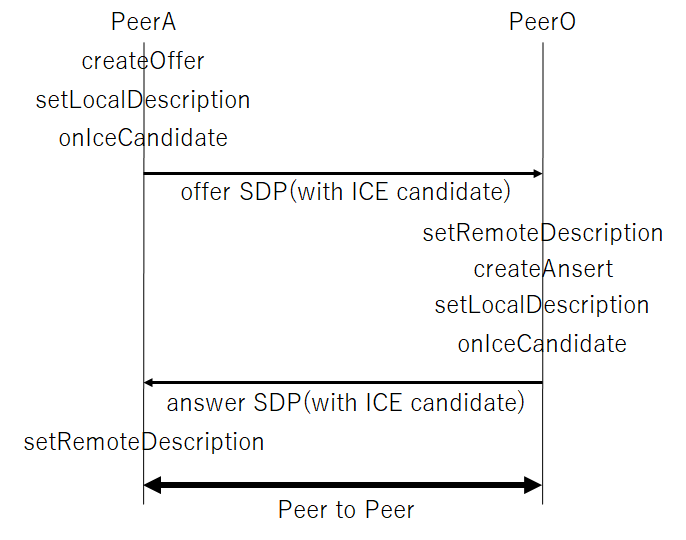
\includegraphics[width=10cm]{./assets/image/signaling.png}
  \caption{シグナリング}
  \label{fig:signaling}
\end{figure}
PeerAがcreateOfferを行いoffer側のSDPの作成準備を行う.
次にsetLocalDescriptionでSDPを作成し,
ICE candidateのリストアップを行う.
ICE candidateのリストアップが完了すると,
ICE candidateをoffer側のSDPの中に含ませて,PeerOへ送る.
PeerOはPeerAのoffer側のSDPをsetRemoteDescriptionで受け取り,
createAnswerでanswer側のSDPの作成準備を行う.
setLocalDescriptionでSDPを作成し,ICE candidateのリストアップを行う.
ICE candidateのリストアップが完了するとICE candidateを
answer側のSDPの中に含ませて,PeerAへ送る.
PeerAはPeerOのanswer側のSDPをsetRemoteDescriptionで受け取りP2P接続が完了する.


\chapter{本論}
\section{手法}



\chapter{おわりに}
\begin{acknowledgment}
	本研究を進めるにあたり, ご指導を頂いた指導教員の萩原助教授に感謝致します.
	日頃の議論において助言や知識を頂いた萩原研究室の皆様に感謝します.
\end{acknowledgment}
\nocite{*}
\bibliographystyle{plain}
\bibliography{reference}
\end{document}
